\documentclass[ngerman,14pt,aspectratio=1610]{beamer}
\usepackage{hyperref}
\hypersetup{breaklinks=true}

% Imports
\usepackage[utf8]{inputenc}
\usepackage[T1]{fontenc}
\usepackage{babel}
\usepackage{graphicx}
\usepackage{multicol}
\usepackage{textpos} % Logo in frametitle
\usepackage{ifthen} % Für das \ifthenelse
\usepackage{totcount} % Für Counter, die in main.aux gespeichert werden

% Startpfad für Bilder setzen
\graphicspath{ {./images/} }

% DHBW Logos
\newcommand{\dhbwlangtrans}{
\includegraphics[width=5cm]{dhbw_lang_trans}}
\newcommand{\dhbwkurzweiss}{
\includegraphics[width=0.5\paperwidth]{dhbw}}

% Subsections zählen
\def\secname{Gliederung} % Der Titel der jeweiligen Section wird in secname gespeichert, damit innerhalb der Section der counter mit dem name erhöht werden kann
\let\oldsection\section
\renewcommand{\section}[1]{
	\oldsection{#1}
	\newtotcounter{#1}
	\def\secname{#1}
}
\let\oldsubsection\subsection
\renewcommand{\subsection}[1]{
	\oldsubsection{#1} 
	\stepcounter{\secname}
}

% Nummern bei Frametitle
\newcommand{\secpagnum}{\insertsectionnumber.\thesubsection}
\newcommand{\lastpagenum}{1}
\let\oldframetitle\frametitle
\renewcommand{\frametitle}[1]{
	\ifthenelse{\equal{\lastpagenum}{\insertslidenumber}}{
		\subsection{}
		\renewcommand{\lastpagenum}{\insertslidenumber}
	}{
		% Hier soll nichts passieren, damit bei gleichen slides der title nicht neu gesetzt wird
	}
	
	\ifthenelse{\totvalue{\secname}>1}{
	\oldframetitle{\secpagnum~#1}
	}{
	\oldframetitle{\insertsectionnumber~#1}
	}
}

% Multicol column balancing ausschalten
\raggedcolumns

% Basis-Theme
\usetheme[progressbar=frametitle, block=fill, sectionpage=none]{metropolis} % Hier kann die progressbar deaktiviert/replaziert werden
\setbeamertemplate{frame numbering}[counter]
\useoutertheme{metropolis}
\useinnertheme{metropolis}
\usefonttheme{metropolis}
\setbeamercolor{background canvas}{bg=white}

% Sections im ToC Nummerieren
\setbeamertemplate{section in toc}[sections numbered]
\setbeamertemplate{subsection in toc}[subsections numbered]

% Zeilenabstand ToC
\makeatletter
\patchcmd{\beamer@sectionintoc}
{\vfill}
{\vskip\itemsep}
{}
{}
\makeatother 

% DHBW Farben
\definecolor{dhbw_grau}{RGB}{93,104,110}
\definecolor{dhbw_rot}{RGB}{227,6,19}
\definecolor{dunkelgrau}{RGB}{41,55,67}
\definecolor{hellgrau}{RGB}{239,241,242}

% DHBW Farben einbauen
\setbeamercolor{progress bar}{fg=dhbw_rot, bg=hellgrau}
\setbeamercolor{normal text}{fg=dunkelgrau} %bg hier macht block bg
\setbeamercolor{alerted text}{fg=dhbw_rot}
\setbeamercolor{frametitle}{fg=dhbw_rot,bg=hellgrau}
\setbeamercolor{title}{fg=dhbw_rot}
\setbeamercolor{subtitle}{fg=dunkelgrau}
\setbeamercolor{section title}{fg=dhbw_rot}
\setbeamercolor{institute}{fg=dhbw_rot}


\setbeamerfont{subtitle}{size=\small}

% Logo in frametitle
\addtobeamertemplate{frametitle}{}{%
	\begin{textblock*}{5cm}(\textwidth-4cm,-1.3cm)
		\dhbwlangtrans
	\end{textblock*}}

% Datum in der Fußzeile
\newcommand{\source}{}
\setbeamertemplate{frame footer}{
	\hskip 2.5em \insertdate \hspace{1em} \source
}

% Endseite
\newcommand{\finalpage}[2][Vielen Dank für ihre Aufmerksamkeit!]{
\metroset{sectionpage=none}
\setbeamertemplate{frame numbering}[none]
\setbeamertemplate{frame footer}{}
\oldsection*{#1}
\begin{frame} \vspace{60pt}
	\sectionpage
	\vspace{10pt}
	\centering
	#2
\end{frame}
}

% Daten für die Titelseite
\title{Einfluss der Teststrategien auf die Daten für die Pandemiesimulation}
\subtitle{Bioinformatik}
\author{Sven Sendke}
\institute[DHBW Stuttgart]{Duale Hochschule Baden-Württemberg Stuttgart}
\date{10.03.2025}	
\titlegraphic { 
	\begin{tikzpicture}[overlay,remember picture]
		\node[right=0.5cm] at (current page.154){
			\dhbwlangtrans
		};
	\end{tikzpicture}
}

\regtotcounter{section}
\regtotcounter{subsection}

\begin{document}
	
	\begin{frame}[plain,noframenumbering]
		\titlepage
	\end{frame}

	\newtotcounter{Gliederung}
	
	\begin{frame}[t]{Gliederung} \vspace{5pt}
		\oldframetitle{Gliederung}
		\begin{columns}[T, onlytextwidth]
			\column{0.5\textwidth}
			\linespread{1.5}
			\tableofcontents
			\column{0.5\textwidth}
		\end{columns}
	\end{frame}
	
	\metroset{sectionpage=simple} % Erst hier definiert, damit die Gliederung keine Sectionpage hat
	
	\section{Allgemeine Einführung}
	
	\renewcommand{\source}{Quelle: \url{https://arxiv.org/pdf/2210.13089}}
	
	\begin{frame}[t]{Covid-19} \vspace{15pt}
		\begin{itemize}
			\item Erstes Covid-19 Jahr $\rightarrow$ Lockdown
			\item \textbf{ABER} Langfristig schwer zu halten $\rightarrow$ wirtschaftliche und psychische Gründe
			\item Vertrauen sinkt, Fake News, Verweigerung oder Zögern beim Impfen
		\end{itemize}
		
		$\rightarrow$ \textbf{Lösung}: Simulation verschiedener Strategien zur Ermittlung optimaler Parameter \\
		Diese Präsentation konzentriert sich auf die \textbf{\alert{Teststrategien}}
	\end{frame}
	
	\section{Teststrategien}
	
	\begin{frame}[t]{Testarten} \vspace{40pt}
			\begin{itemize}
				\item PCR tests
				\item Serological tests
				\item Antigenic tests
				\item Auto-tests
			\end{itemize}
			
			$\rightarrow$  Alle verschiedene Qualitätslevel
	\end{frame}
	
	\renewcommand{\source}{Quelle: \url{https://arxiv.org/pdf/2210.13089}}
	
	\begin{frame}[t]{Qualitätslevel}
		\only<1>{
		\begin{figure}[h]
			\centering
			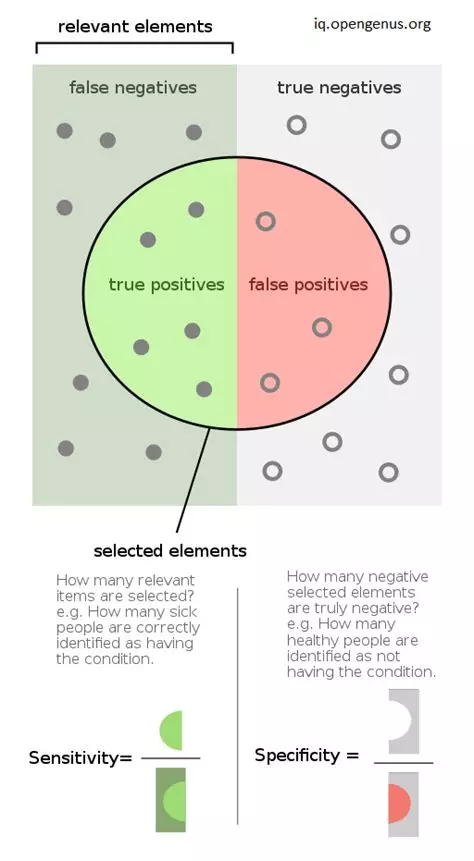
\includegraphics[width=0.28\linewidth]{sensitivity-specificity}
			\tiny Quelle: \href{https://iq.opengenus.org/precision-recall-sensitivity-specificity/}{\texttt{https://iq.opengenus.org}}
		\end{figure}
	}
	
	\only<2>{
		\vspace{5pt}
		\begin{itemize}
			\item \textbf{\alert{Sensitivität:}} Wahrscheinlichkeit, dass ein Test bei kranken Personen positiv ist
			\begin{itemize}
				\item 100\% Sensitivität $\rightarrow$ keine falschen Negativen
			\end{itemize}
			
			\item \textbf{\alert{Spezifität:}} Wahrscheinlichkeit, dass ein Test bei gesunden Personen negativ ist
			\begin{itemize}
				\item 100\% Spezifität $\rightarrow$ keine falschen Positiven
			\end{itemize}
		
			\item \textbf{Kein perfekter Test:}
			\begin{itemize}
				\item \textbf{Hohe Sensitivität} $\rightarrow$ Weniger falsche Negative \\ $\rightarrow$ Infizierte werden erkannt und isoliert
				\item \textbf{Hohe Spezifität} $\rightarrow$ Weniger falsche Positive \\ $\rightarrow$ Gesunde werden nicht unnötig isoliert
			\end{itemize}
		\end{itemize}
	}
	\end{frame}
	
	\begin{frame}[t]{Teststrategien} \vspace{40pt}
		\begin{itemize}
			\item Wer soll priorisiert getestet werden?
			\item Vergleich von Teststrategien:
			\begin{itemize}
				\item Zufällige Tests
				\item Testen von symptomatischen Personen
				\item Testen von Hochrisikogruppen
				\item Testen von Personen mit vielen Kontakten
			\end{itemize}
		\end{itemize}
	\end{frame}
	
	\section{Bezug zum Paper}
	
	\renewcommand{\source}{ }
	
	\begin{frame}[t]{Relevanz des Themas} \vspace{5pt}
		\begin{itemize}
			\item Paper behandelt die Simulation von Teststrategien für Pandemien
			\item Ziel: Analyse der Auswirkungen verschiedener Testmethoden auf die Eindämmung der Pandemie
			\item Warum relevant?
			\begin{itemize}
				\item Optimierung von Teststrategien kann Ausbreitung minimieren
				\item Hilft politischen Entscheidungsträgern bei der Planung
				\item Verbindung zu realen Szenarien (z. B. COVID-19)
			\end{itemize}
			\item \textbf{\alert{Ziel dieser Präsentation}} $\rightarrow$ Simulationsergebnisse und deren Implikationen
		\end{itemize}
	\end{frame}
	
	\renewcommand{\source}{Quelle: \url{https://arxiv.org/pdf/2210.13089}}
	
	\begin{frame}[t]{Vorteile von Simulationen} \vspace{10pt}
		\begin{itemize}
			\item Vergleich von Strategien unter \textbf{gleichen Bedingungen}
			\item Exakt gleiche Szenarien mit \textbf{veränderten Parametern}
			\item Die \textbf{tatsächliche} Infektionskurve kann mit der \textbf{geschätzten verglichen} werden
			\item Unvorhergesehene Folgen von Maßnahmen können \textbf{frühzeitig} erkannt werden
			\item Ermöglicht die Optimierung von (Impf- und) Teststrategien, um \textbf{effektive Maßnahmen} abzuleiten
		\end{itemize}
	\end{frame}
	
	\section{Wissenschaftliche Beispiele}
	
	\begin{frame}[t]{Belege aus Forschung und Praxis} \vspace{5pt}
		\begin{itemize}
			\item \href{https://www.ssoar.info/ssoar/bitstream/handle/document/82820/sopolis-die-simulation-der-pandemie.pdf?sequence=-1&isAllowed=y&lnkname=sopolis-die-simulation-der-pandemie.pdf}{\texttt{Die Simulation der Pandemie}}: Diese Studie befasst sich mit der Rolle von Computersimulationen in der Pandemiebewältigung.
			\item \href{https://www.nature.com/articles/s43588-021-00031-0}{\texttt{Quantifying the uncertainty of CovidSim}}: Untersuchung von Covid-Simulationen $\rightarrow$ Bewertung der Auswirkungen von Unsicherheiten auf die Modellergebnisse
			\item Praktische Anwendung: COVID-19-Strategien vieler Länder basierten auf ähnlichen Modellierungen. In dem Paper wird Frankreich als Beispiel benannt.
		\end{itemize}
	\end{frame}
	
	\section{Implementierung}
	
	\renewcommand{\source}{ }
	
	\begin{frame}[t]{Agentenbasierte Simulation} \vspace{30pt}		
		\begin{columns}[T, onlytextwidth]
			\column{0.45\textwidth}
			\begin{itemize}
				\item Implementierung in NetLogo
				\item Simulation verschiedener Teststrategien
				\item Parameter: Testverfügbarkeit, Startzeitpunkt, Zielgruppe
			\end{itemize}
			
			\column{0.45\textwidth}			
			\begin{figure}[h]
				\centering
				
\includegraphics[width=\linewidth]{netlogo}
				\tiny Quelle: \href{https://www.upwork.com/services/product/development-it-a-netlogo-agent-based-simulation-model-1351194777425215488}{\texttt{https://www.upwork.com}}
			\end{figure}
			
		\end{columns}
	\end{frame}
	
	\begin{frame}[t]{Praxisbeispiele} \vspace{60pt}
		\textbf{\textit{Aber nun genug von der Theorie...}}\\
		\bigskip
		\url{https://nausikaa.net/wp-content/uploads/2022/10/virus1-screening-en.html}
	\end{frame}
	
	\renewcommand{\source}{Quelle: \url{https://arxiv.org/pdf/2210.13089}}
	
	\begin{frame}[t]{Erkenntnisse}
		\begin{itemize}
			\item Wahl der Teststrategie beeinflusst die Wahrnehmung der Epidemie \textbf{erheblich}
			\item \textbf{\alert{Zufällige Tests}}: liefern \textbf{genauere Schätzungen}, aber \textbf{„verschwenden“ viele Tests} an nicht infizierte Personen
			\item \textbf{\alert{Symptomatischen Personen}}: führt zu einer \textbf{Überschätzung} der Infektionszahlen
			\item \textbf{\alert{Hochrisikogruppen}} oder \textbf{\alert{Personen mit vielen Kontakten}}: kann effektiver sein, erzeugt aber \textbf{Verzerrungen}
			\item \textbf{Früher Start} der Testkampagne \textbf{verbessert die Kontrolle} der Epidemie erheblich
		\end{itemize}
	\end{frame}
	
	\section{Schluss}
		\renewcommand{\source}{ }
	
		\begin{frame}[t]{Überraschenste Erkenntnis} \vspace{80pt}
			 Wenn nur symptomatische Personen getestet werden, wird die Gesamtzahl der Infektionen in der Bevölkerung erheblich überschätzt.
		\end{frame}
		
		\begin{frame}[t]{Zusammenfassung} \vspace{15pt}
			\begin{itemize}
				\item \textbf{Einführung:} COVID-19-Lockdowns und deren Herausforderungen. Simulationen optimieren Teststrategien.
				\item \textbf{Teststrategien:} Verschiedene Testarten und Qualitätslevels (Sensitivität und Spezifität).
				\item \textbf{Relevanz:} Simulationen unterstützen politische Entscheidungen und Pandemiebewältigung.
				\item \textbf{Erkenntnisse:} Teststrategie beeinflusst Epidemiewahrnehmung. Früher Teststart verbessert Kontrolle.
			\end{itemize}
		\end{frame}
	
	\section{Fragen}
	
		\begin{frame}[t]{Fragen} \vspace{85pt}
			\centering
			\textbf{Gibt es irgendwelche Fragen?}
		\end{frame}	
		
		\begin{frame}[t]{Frage 1} \vspace{20pt}
			\textbf{Was beschreibt die Sensitivität eines Tests?}
			\begin{enumerate}
				\item[A] Die Wahrscheinlichkeit, dass ein Test bei gesunden Personen negativ ist
				\only<1>{\item [B] Die Wahrscheinlichkeit, dass ein Test bei kranken Personen positiv ist}
				\only<2>{\item[B] \textbf{\alert{Die Wahrscheinlichkeit, dass ein Test bei kranken Personen positiv ist}}}
				\item[C] Die Genauigkeit eines Tests in Bezug auf alle getesteten Personen
				\item[D] Die Anzahl der durchgeführten Tests pro Tag
			\end{enumerate}
		\end{frame}
		
		\begin{frame}[t]{Frage 2} \vspace{40pt}
			\textbf{Warum ist ein früher Start der Testkampagne vorteilhaft?}
			\begin{enumerate}
				\item[A] Weil weniger Tests benötigt werden
				\item[B] Weil die Tests dann eine höhere Genauigkeit haben
				\only<1>{\item[C] Weil die Epidemie dadurch besser kontrolliert werden kann}
				\only<2>{\item[C] \textbf{\alert{Weil die Epidemie dadurch besser kontrolliert werden kann }}}
				\item[D] Weil dadurch keine Verzerrungen mehr auftreten
			\end{enumerate}
		\end{frame}
		
		\begin{frame}[t]{Frage 3} \vspace{20pt}
			\textbf{Welche Teststrategie liefert genauere Schätzungen, „verschwendet“ aber viele Tests an nicht infizierte Personen?}
			\begin{enumerate}
				\item[A] Testen von symptomatischen Personen
				\item[B] Testen von Hochrisikogruppen
				\only<1>{\item[C] Zufällige Tests }
				\only<2>{\item[C] \textbf{\alert{Zufällige Tests }}}
				\item[D] Testen von Personen mit vielen Kontakten
			\end{enumerate}
		\end{frame}
	
	\finalpage{\inserttitlegraphic}
	%\frame{\sectionpage}

\end{document}